\subsubsection{Continental extension}
\label{sec:cookbooks-continental-extension}
\textit{This section was contributed by John Naliboff, Anne Glerum, and Valentina Magni}

In the crustal deformation examples above, the viscosity depends solely on the Drucker Prager yield criterion defined by the cohesion and internal friction angle. While this approximation works reasonably well for the uppermost crust, deeper portions of the lithosphere may undergo either brittle or viscous deformation, with the latter depending on a combination of composition, temperature, pressure and strain-rate. In effect, a combination of the Drucker-Prager and Diffusion dislocation material models is required. The visco-plastic material model is designed to take into account both brittle (plastic) and non-linear viscous deformation, thus providing a template for modeling complex lithospheric processes. Such a material model can be used in \aspect{} using the following set of input parameters:

\lstinputlisting[language=prmfile]{cookbooks/continental_extension/doc/continental_extension_material_model.prm.out}

This cookbook provides one such example where the continental lithosphere undergoes extension. Notably, the model design follows that of numerous previously published continental extension studies~\cite[and references therein]{Hui11,Bru14,Nal15}.

\paragraph{Continental Extension}
The 2D Cartesian model spans 200 ($x$) by 100 ($y$) km and has a finite element grid with 1.25 and 2.5 km grid spacing, respectively, above and  below 50 km depth. This variation in grid spacing is achieved with a single initial adaptive refinement step using the minimum refinement function strategy. Unlike the crustal deformation cookbook (see Section~\ref{sec:cookbooks-crustal-deformation}, the mesh is not refined with time.

\lstinputlisting[language=prmfile]{cookbooks/continental_extension/doc/continental_extension_geometry_mesh.prm.out}


Similar to the crustal deformation examples above, this model contains a free surface. However, in this example the free surface is advected using the full velocity (e.g., normal projection) rather than only the vertical component. As this projection can lead to signficant surface mesh deformation and associated solver convergence issues, diffusion is applied to the free surface at each time step. Deformation is driven by constant horizontal ($x$-component) velocities (0.25 cm/yr) on the side boundaries ($y$-velocity component unconstrained), while the bottom boundary has vertical inflow to balance the lateral outflow. The top, and bottom boundaries have fixed temperatures, while the sides are insulating. The bottom boundary is also assigned a fixed composition, while the top and sides are unconstrained.

\lstinputlisting[language=prmfile]{cookbooks/continental_extension/doc/continental_extension_boundary_conditions.prm.out}

Sections of the lithosphere with distinct properties are represented by compositional fields for the upper crust (20 km thick), lower crust (20 km thick) and mantle lithosphere (60 km thick). Material (viscous flow law parameters, cohesion, internal friction angle) and thermodynamic properties for each compositional field are based largely on previous numerical studies. Dislocation creep viscous flow parameters are taken from published deformation experiments for wet quartzite \cite{RB04}, wet anorthite \cite{RGWD06} and dry olivine \cite{HK04}. Additional compositional fields are used to track plastic strain and the non-initial plastic strain, with the latter value tracking the same quantity as the plastic strain absent the initial plastic strain values. As discussed further on, the plastic strain is used to soften (e.g., reduce) the friction and cohesion through time based on user-specified bounds and magnitudes. The initial randomized values of plastic strain in the model center localize distributed deformation in this region.

\lstinputlisting[language=prmfile]{cookbooks/continental_extension/doc/continental_extension_composition.prm.out}

The initial thermal structure, radiogenic heating model and associated thermal properties are consistent with the prescribed thermal boundary conditions and produce a geotherm characteristic of the continental lithosphere. The equations defining the initial geotherm \cite{Cha86} follow the form
\begin{align}
  \label{eq:continental-geotherm-1}
  T(z) &= T_T + \frac{q_T}{k}z - \frac{Az^2}{2k}
\end{align}
where $T$ is temperature, $z$ is depth, $T_T$ is the temperature at the layer surface (top), $q_T$ is surface heat flux, $k$ is thermal conductivity, and $A$ is radiogenic heat production.

For a layer thickness $\Delta z$, the basal temperature ($T_B$) and heat flux ($q_B$) are
\begin{align}
  \label{eq:continental-geotherm-2}
  T_B &= T_T + \frac{q_T}{k} \Delta z - \frac{A \Delta z^2}{2k},
  \\
  \label{eq:continental-geotherm-3}
  q_B &= q_T - A \Delta z.
\end{align}

In this example, specifying the top (\SI{273}{K}) temperature, surface heat flow (\SI{55}{\milli\watt\per\meter^2}), and thermal conductivity and radiogenic heat production of each layer provides enough constraints to successively solve for the temperature and heat flux at the top of the lower crust and mantle.

As noted above, the initial zone of randomized plastic strain within the model center and strain softening of the friction and cohesion produces an initial pattern of distributed and unlocalized deformation across the zone of initial plastic strain (Fig.~\ref{fig:continental_extension_cookbook_0myr}). After 5 million years of extension, distributed faulting is clearly evident in both the active and finite deformation fields and surface topography over an approximately 100 km wide region (Fig.~\ref{fig:continental_extension_cookbook_5myr}). While deformation is distributed within this region, the fault system is clearly asymmetric as the rate of deformation and accumulated brittle strain varies between faults. Localization onto the two conjugate rift-bounding border faults is evident from the active deformation field. Notably, deformation of the free surface near the fixed left and right walls is evident at 5 Myr. Continued distortion of the surface mesh near the lateral boundaries may lead to solver issues, which can be overcome by either widening the model or allowing the mesh to deform along these boundaries.  

With further extension for millions of years, significant crustal thinning and surface topography development should occur in response to displacement along the rift-bounding faults. However, given that the model only extends to 100 km depth, the simulation will not produce a realistic representation of continental breakup due to the lack of an upwelling asthenosphere layer. Indeed, numerical studies that examine continental breakup, rather than just the initial stages of continental extension, include an asthenospheric layer or modified basal boundary conditions (e.g. Winkler boundary condition \cite[for example]{Bru14}) as temperature variations associated with lithospheric thinning exert a first-order influence on the deformation patterns. As noted below, numerous additional parameters may also affect the temporal evolution of deformation patterns.

\note{It is important to consider that the non-linearity of visco-plastic rheologies and mesh-dependence of brittle shear bands make lithospheric deformation models highly sensitive to a large number of parameters. In order to ensure the conclusions drawn from a series of numerical experiments are robust, one should complete a sensitivity test for a large range of parameters including grid resolution, model geometry, boundary conditions, initial composition and temperature conditions, material properties, composition discretization, CFL number and solver settings. If you are new to modeling lithospheric processes, a reasonable starting point is to try and reproduce results from a relevant previous study and then perform a sensitivity test for the parameters listed above. While highly time consuming, completing this procedure will prove invaluable when you design and assess the results of your own numerical study.}

\begin{figure}
\centering
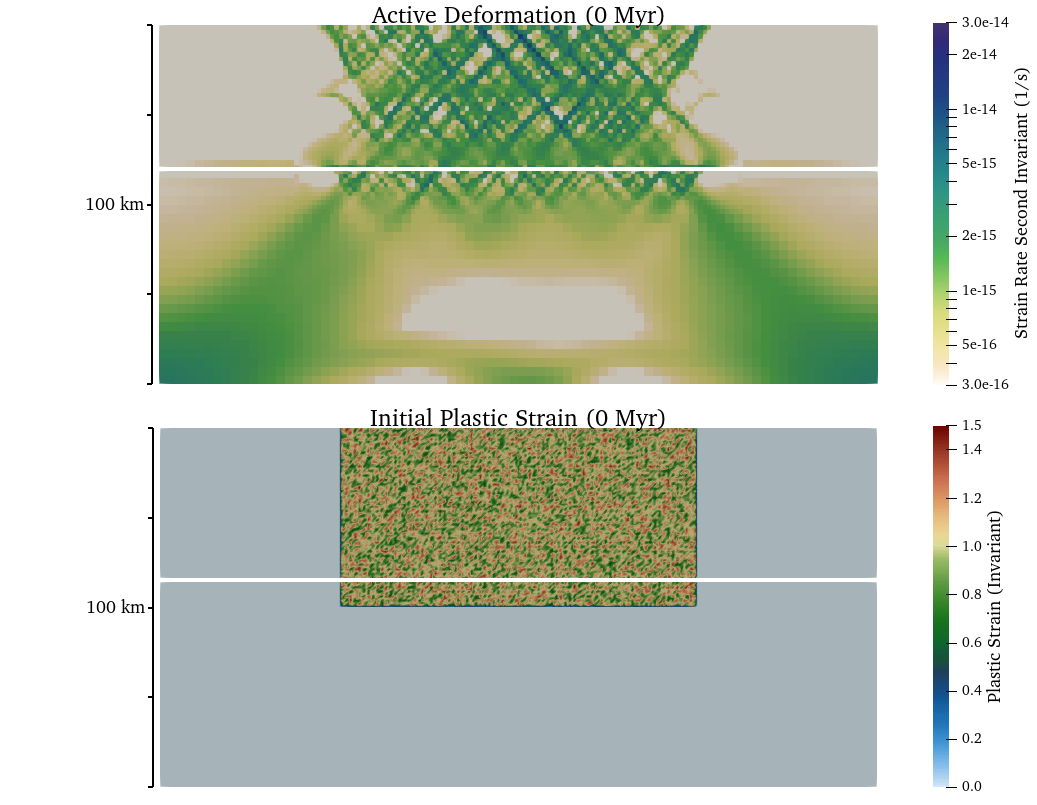
\includegraphics[width=\textwidth]{cookbooks/continental_extension/doc/continental_extension_cookbook_0myr.png}
\caption{\it Initial active deformation field (strain rate second invariant in units of $\si{s}^{-1}$) and distribution of plastic strain. The white line marks the (\SI{893}{K}) isotherm (initial Moho temperature).}
\label{fig:continental_extension_cookbook_0myr}
\end{figure}
\begin{figure}
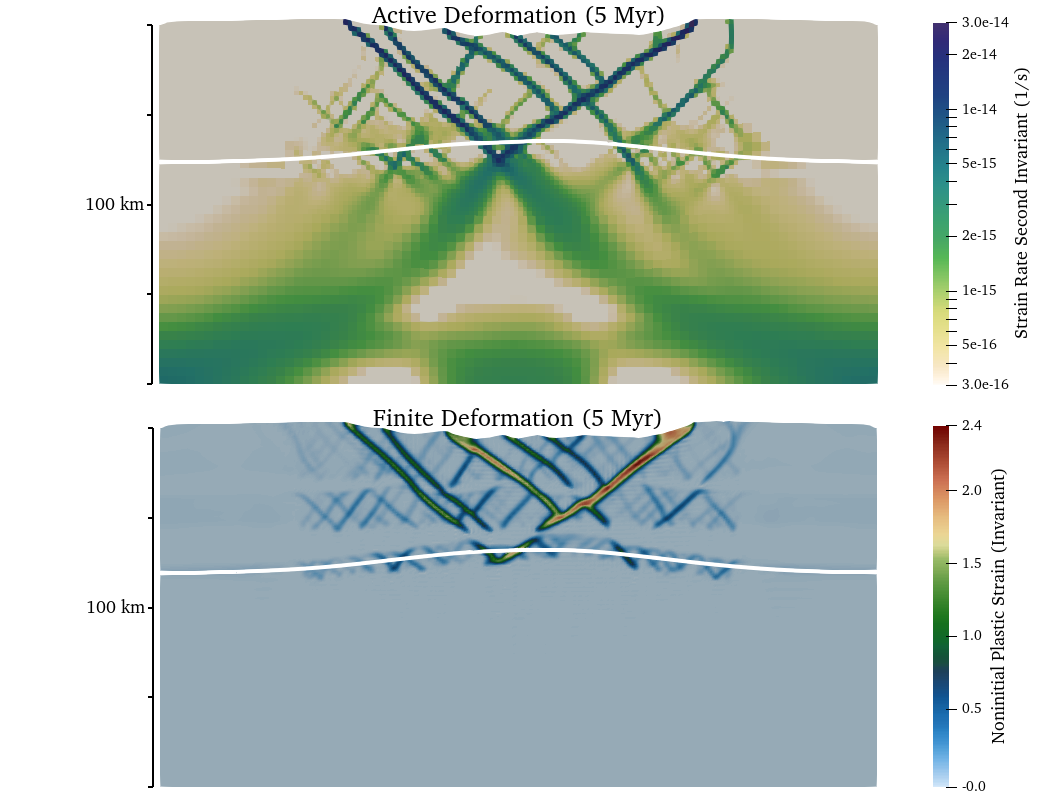
\includegraphics[width=\textwidth]{cookbooks/continental_extension/doc/continental_extension_cookbook_5myr.png}
\caption{\it Active (strain rate second invariant in units of $\si{s}^{-1}$) and finite (plastic) deformation after \num{5e6} years of extension. The white line marks the (\SI{893}{K}) isotherm (initial Moho temperature).}
\label{fig:continental_extension_cookbook_5myr}
\end{figure}
